\documentclass{article}
    \usepackage{amssymb}
    \usepackage{color}
    \usepackage{listings}
    \usepackage{graphicx}
    \usepackage{subcaption}
    \usepackage{geometry}
    \usepackage{float}
    \geometry{
    a4paper,
    total={170mm,257mm},
    left=20mm,
    top=20mm,
    }
    
    \setlength{\parindent}{0em}
    \setlength{\parskip}{1em} % length of the spacing
    
    \lstset{ % General setup for the package
        language=Python,
        basicstyle=\small\sffamily,
        numbers=left,
        numberstyle=\tiny,
        frame=tb,
        tabsize=4,
        columns=fixed,
        showstringspaces=false,
        showtabs=false,
        keepspaces,
        commentstyle=\color{red},
        keywordstyle=\color{blue},
        emphstyle=\ttb\color{deepred},    
        stringstyle=\color{deepgreen}
    }
    
    \begin{document}
        \begin{figure}
            \centering
            
\includegraphics[width=0.5\linewidth]{./img/vub.png}
        \end{figure}
        \title{Navigation and Intelligent Vehicles, Lab session 2 Report}
        \author{Juan Jose Soriano Escobar }
        \maketitle
        \newpage

        \section{Simulated measurement data}
        
        This practical session is a little bit different as the first one in the sense that
        this time we are trying to estimate or to "keep track" of the movement of  an object
        or particle in one given dimension (1-D) with an unpredicted acceleration that could be
        also interpreted as a noise.
        
        In order to simulate the data measurement, it is necessary first to define the movement of
        the particle by a mathematical model as is describe in the equation \ref{eq:1} where the position
        \textbf{\textit{x}} depends on the previous position and velocity plus the noise \textbf{\textit{w}}
        that is given by changes of the acceleration in a given moment for an specific direction.

        \begin{equation}\label{eq:1}
            x(k + 1) = Ax(k) + Gw(k) 
        \end{equation}

        Once the movement of the particle is explained, it is needed to find a way to measure the position of 
        the particle in order to compare and correct the predicted value. The measurement function is given by
        the \ref{eq:2}, which contains \textbf{\textit{x}} as the current movement model of the particle + \textbf{\textit{v}}
        functions that is the noise in the measurement of the position (variable of interest) of the particle in a time 
        \textbf{\textit{k}}.

        \begin{equation}\label{eq:2}
            z(k) = Cx(k) + Hv(k)
        \end{equation}\label{eq:2}

        With the mathematical model defined, it is important to express the generation of the data on a emulated system
        to play with the variables and visualize the results. For this project I used again python and the simulated data is expressed
        in the listing \ref{lst:data}

        \begin{lstlisting}[language=Python, caption= Data Generation, label={lst:data}]
            data = []
            Xk = np.matrix([[0.0],[10.0]])

            def simulate_movement(A, X, q):            
            process_model = np.dot(A, X) + 
                            np.matrix([[np.random.normal(0, np.sqrt(q*((dt**3)/3)))], 
                            [np.random.normal(0, np.sqrt(q*dt))]]) 
            return process_model
            
            for i in range(100):
                data.append(Xk)
                Xk = simulate_movement(A, Xk, q)
        \end{lstlisting}

        With the simulated data I proceeded to implement the same logic of the Kalman filter implemented in
        the first practical session, with a Prediction and Update function \ref{lst:functions}. With the only exception that in this
        case our X of interest is a vector with the position and velocity of the particle in movement.  

        \begin{lstlisting}[language=Python, caption= Prediction/Update Kalman function, label={lst:functions}]
            def prediction(X, P, A, Q, B, U):
                X = np.dot(A, X) 
                P = np.dot(A, np.dot(P, A.T)) + Q 
                return (X, P)
            
            def update(X, P, H, Y, R):
                MP = np.dot(H, X) # measurement prediction
                residual = Y - MP # the residual of the prediction
                MPC = np.dot(H, np.dot(P, H.T))  +  r  
                K = np.dot(P, np.dot(H.T, MPC**-1)) # kalman
                X = X + np.dot(K, residual) # Updated State Estimate 
                P = np.dot((np.identity(P.shape[0]) - np.dot(K, H)), P) # Updated P
            
                return (X,P,K)
        \end{lstlisting}

        \section{Single Simulation}
            \subsection{Matched Model}

            The goal in this implementation is to variate \textbf{\textit{q}} (acceleration or process variance) for 3 specific values [0, 1, 9]
            as part of the noise or unpredicted move of the particle. The idea behind the matched model is to use the same \textbf{\textit{q}} for the
            data generation as for the covariance prediction in \textbf{\textit{P}}.

            Due to the random noise every simulation generates a unique movement pattern in the particle. In the figure \ref{fig:movement} is illustrated
            some f the results from the prediction and the real movement for different \textbf{\textit{q}} values.
                
        \begin{figure}[H]
            \begin{subfigure} {.3\textwidth}  
                \centering 
                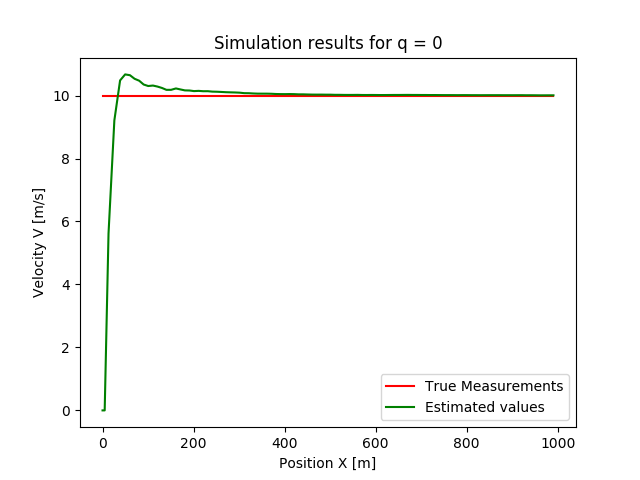
\includegraphics[width=0.9\linewidth]{./img/q_0.png}
                \caption{q = 0 }
            \end{subfigure}
            \begin{subfigure}{.3\textwidth}            
                \centering
                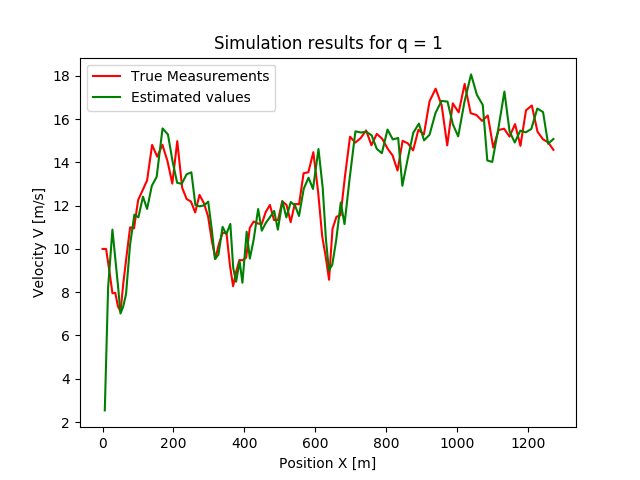
\includegraphics[width=0.9\linewidth]{./img/q_1.png}
                \caption{q = 1}
            \end{subfigure}    
            \begin{subfigure} {.3\textwidth}         
                \centering
                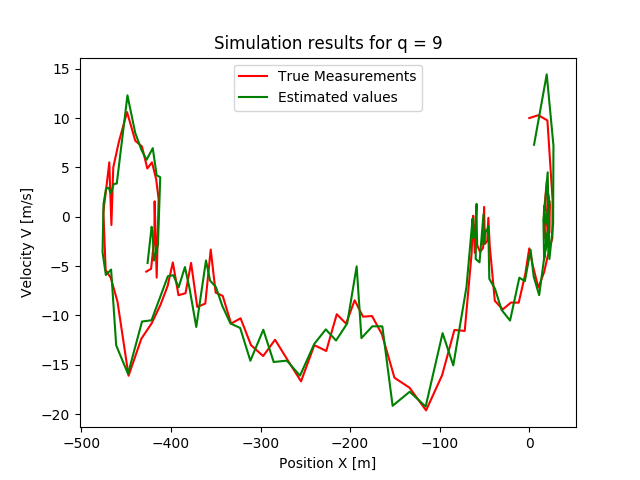
\includegraphics[width=0.9\linewidth]{./img/q_9.png}
                \caption{q = 9}
            \end{subfigure}
            \caption{Simulation for different variance in the movement [0, 1, 9]}
            \label{fig:movement}
        \end{figure}

        In the image \textit{(a)} from the figure \ref{fig:movement}, is a uniform movement without any acceleration with a constant
        velocity of 10 m/s. It is visible how the particle prediction starts in the position (0, 0) and take few iterations to adapt 
        to the real movement and realize about the constant moment of the particle. This will be explained in more detail in the the 
        gain and variance prediction analysis.

        On the other hand, \textit{(b)} and \textit{(c)} describes movement with random generated positive or negative acceleration,
        where the particle is able to move in both directions of the axis if the acceleration is high enough  to overtake the previous momentum and
        velocity of the particle. For example in \textit{(c)} is shown hoe the particle starts in the position 0, towards a "negative" position and
        then in the position -450m it accelerates in the "positive" direction reaching the position -412m at the end of the simulation.

        The learning or adaptation model from the Kalman filter is clearly visible in the prediction \textit{P} and consequently in the kalman gain \textit{K} 
        presented in the Figure \ref{fig:variances} and \ref{fig:kalman}.

        As mentioned before, when the movement is a constant without any acceleration, the variance of \textit{P} for the distance drops exponentially while it
        adapts the initial velocity of 0m/s to the 10m/s up to a variance of almost 0 predicting the value with a high precision. This behavior is also supported
        and visible in the Kalman Gain both for the position and the velocity.
        
        % p measurement
        \begin{figure}[H]
            \centering 
            \begin{subfigure}{1\textwidth}  
                \begin{subfigure}{.3\textwidth}  
                    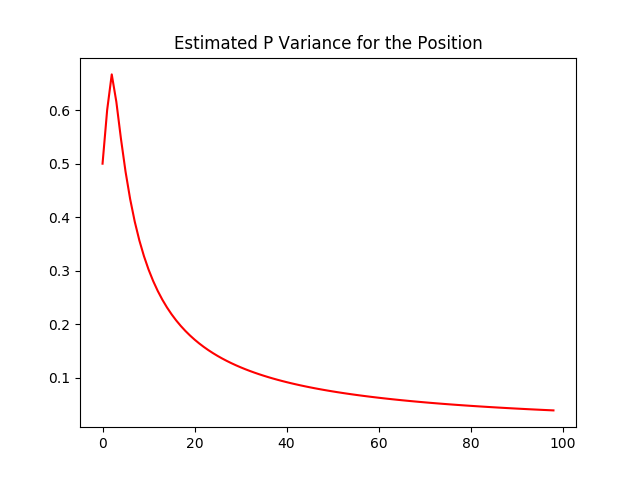
\includegraphics[width=1\linewidth]{./img/p11_0.png}
                    \caption{P11 \& q = 0 }
                \end{subfigure}
                \begin{subfigure}{.3\textwidth}  
                    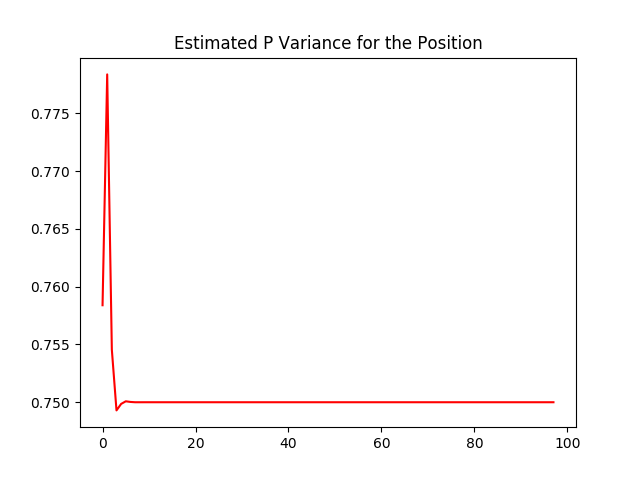
\includegraphics[width=1\linewidth]{./img/p11_1.png}
                    \caption{P11 \& q = 1 }
                \end{subfigure}
                \begin{subfigure}{.3\textwidth}  
                    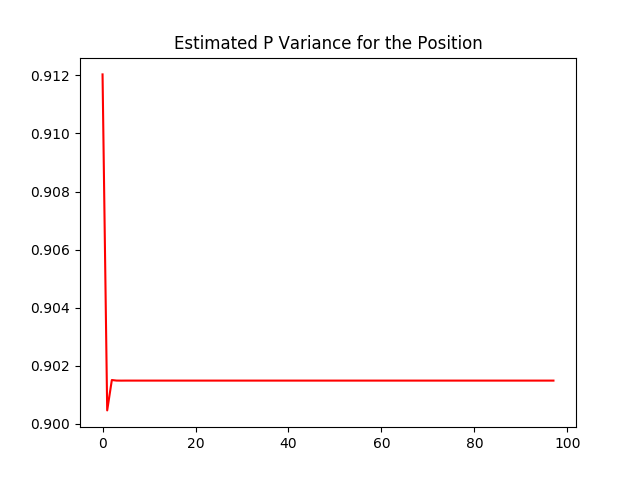
\includegraphics[width=1\linewidth]{./img/p11_9.png}
                    \caption[font=0.1mm]{P11 \& q = 9 }
                \end{subfigure}
            \end{subfigure}
            \begin{subfigure} {1\textwidth}    
                \begin{subfigure}{.3\textwidth}  
                    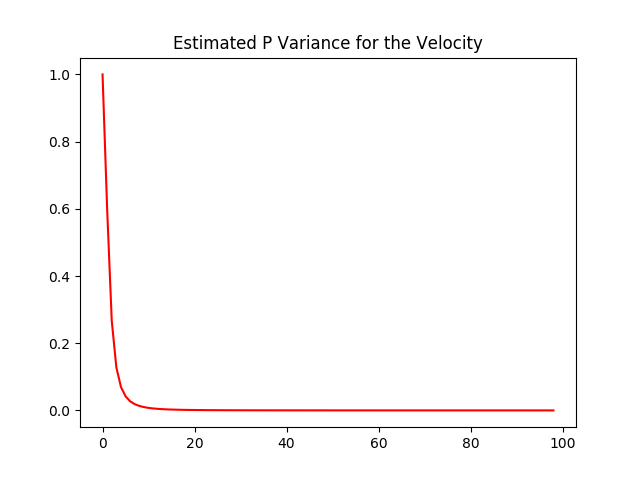
\includegraphics[width=1\linewidth]{./img/p22_0.png}
                    \caption{P22 \& q = 0 }
                \end{subfigure}
                \begin{subfigure}{.3\textwidth}  
                    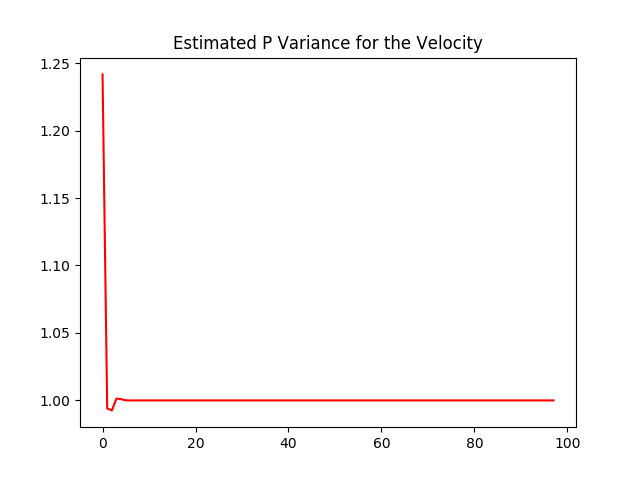
\includegraphics[width=1\linewidth]{./img/p22_1.png}
                    \caption{P22 \& q = 1 }
                \end{subfigure}
                \begin{subfigure}{.3\textwidth}
                    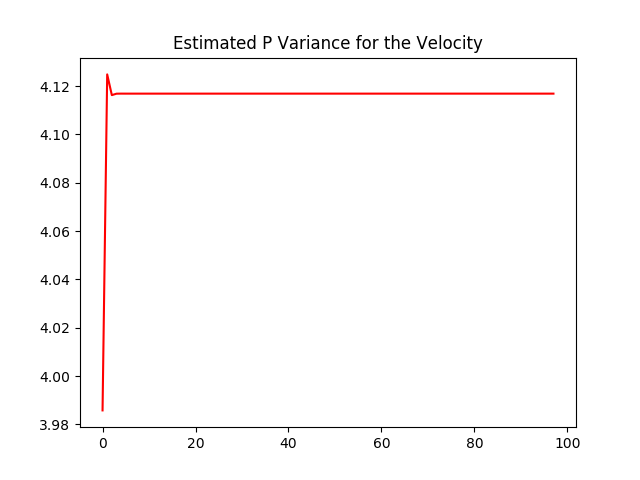
\includegraphics[width=1\linewidth]{./img/p22_9.png}
                    \caption{P22 \& q = 9 }
                \end{subfigure}
            \end{subfigure} 
            \caption{State Covariance P for diffetent q values [0, 1, 9]}
            \label{fig:variances}
        \end{figure}

        % K measurement
        \begin{figure}[H]
            \centering 
            \begin{subfigure}{1\textwidth}  
                \begin{subfigure}{.3\textwidth}  
                    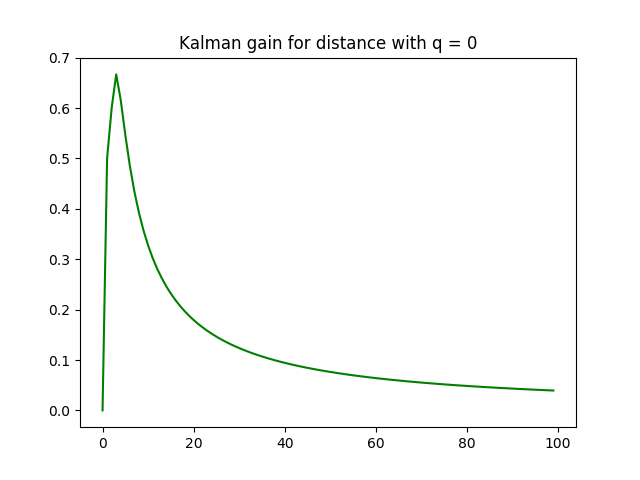
\includegraphics[width=1\linewidth]{./img/k11_0.png}
                    \caption{Kp \& q = 0 }
                \end{subfigure}
                \begin{subfigure}{.3\textwidth}  
                    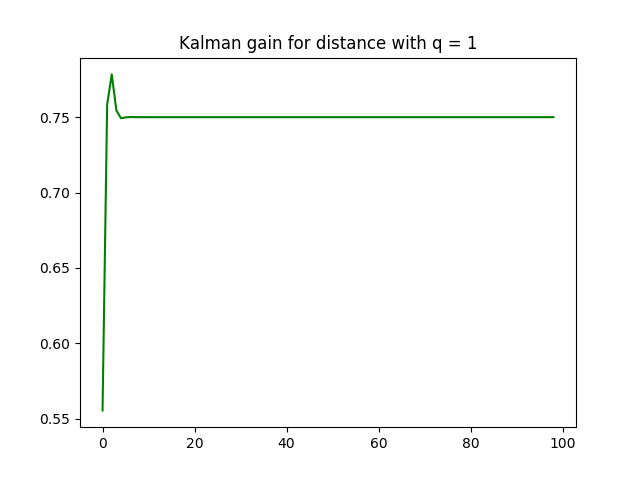
\includegraphics[width=1\linewidth]{./img/k11_1.png}
                    \caption{Kp \& q = 1 }
                \end{subfigure}
                \begin{subfigure}{.3\textwidth}  
                    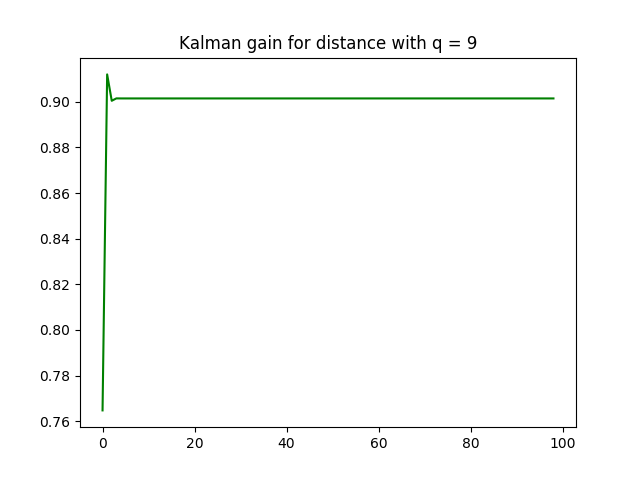
\includegraphics[width=1\linewidth]{./img/k11_9.png}
                    \caption[font=0.1mm]{Kp \& q = 9 }
                \end{subfigure}
            \end{subfigure}
            \begin{subfigure} {1\textwidth}    
                \begin{subfigure}{.3\textwidth}  
                    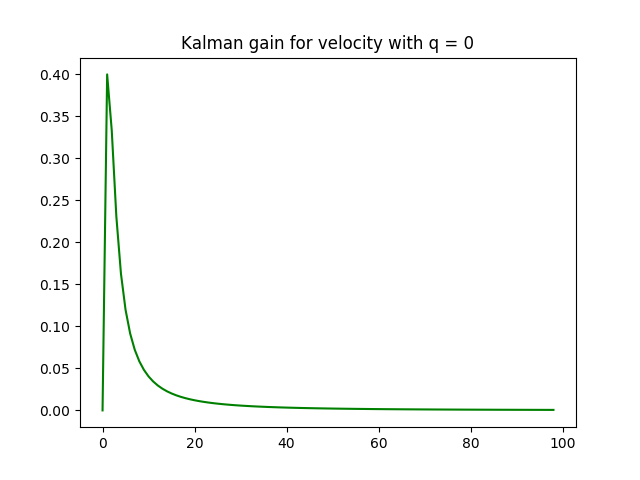
\includegraphics[width=1\linewidth]{./img/k22_0.png}
                    \caption{Kv \& q = 0 }
                \end{subfigure}
                \begin{subfigure}{.3\textwidth}  
                    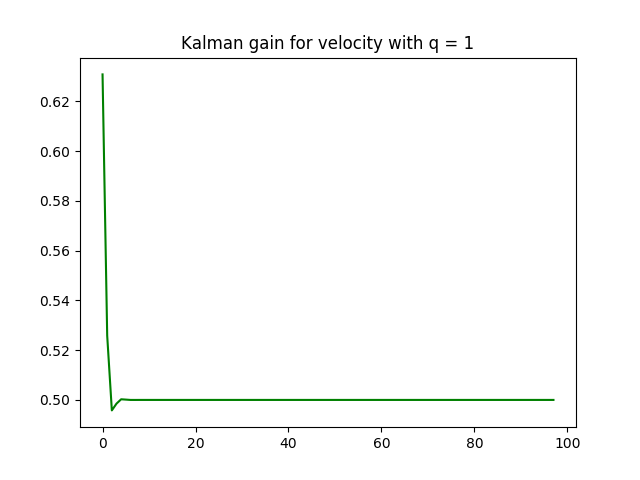
\includegraphics[width=1\linewidth]{./img/k22_1.png}
                    \caption{Kv \& q = 1 }
                \end{subfigure}
                \begin{subfigure}{.3\textwidth}
                    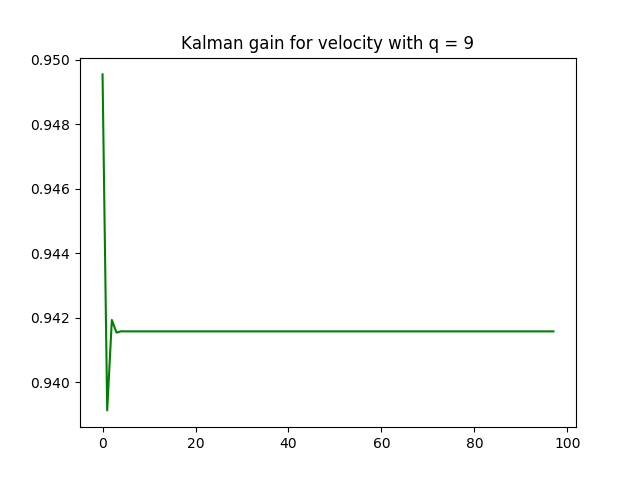
\includegraphics[width=1\linewidth]{./img/k22_9.png}
                    \caption{Kv \& q = 9 }
                \end{subfigure}
            \end{subfigure} 
            \caption{Kalman gain for different q values [0, 1, 9]}
            \label{fig:kalman}
        \end{figure}

        Regarding to the Kalman filter and P for the case of a variance of 1 and 9 for the acceleration,
        it shows a big initial jump while it leaves the initial state to follow the real movement equation.
        The only difference in both cases the convergence variance is bigger due to the higher noise or acceleration the equation.

        % NEES and NIS results
        \begin{figure}[H]
            \centering 
            \begin{subfigure}{1\textwidth}  
                \begin{subfigure}{.3\textwidth}  
                    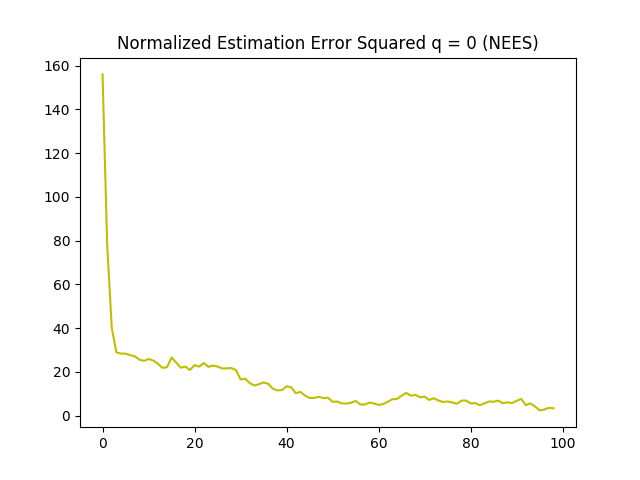
\includegraphics[width=1\linewidth]{./img/nees_0.png}
                    \caption{NEES, q = 0 }
                \end{subfigure}
                \begin{subfigure}{.3\textwidth}  
                    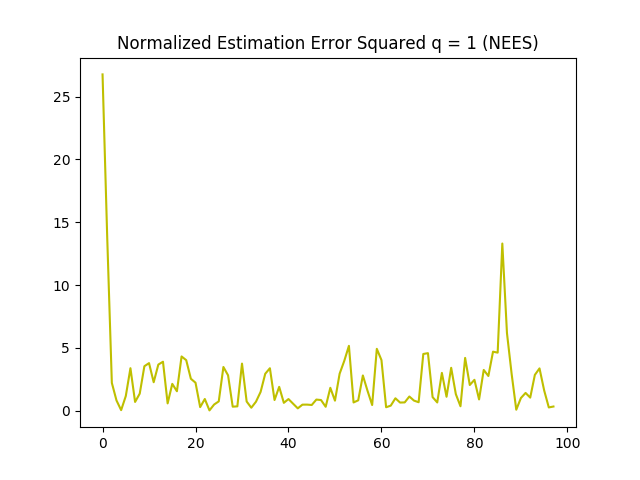
\includegraphics[width=1\linewidth]{./img/nees_1.png}
                    \caption{NEES, q = 1 }
                \end{subfigure}
                \begin{subfigure}{.3\textwidth}  
                    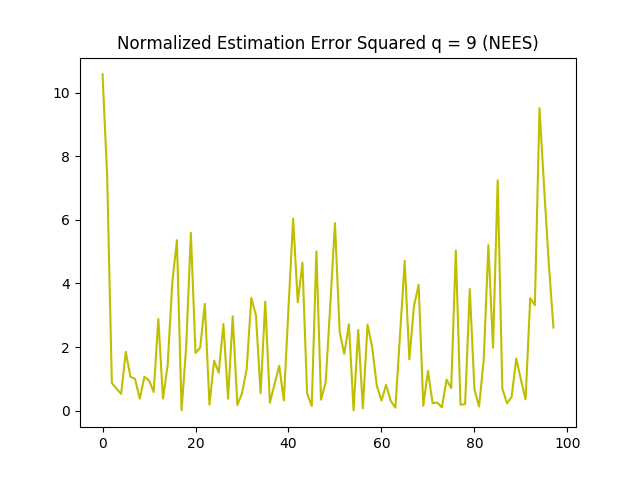
\includegraphics[width=1\linewidth]{./img/nees_9.png}
                    \caption[font=0.1mm]{NEES, q = 9 }
                \end{subfigure}
            \end{subfigure}
            \begin{subfigure} {1\textwidth}    
                \begin{subfigure}{.3\textwidth}  
                    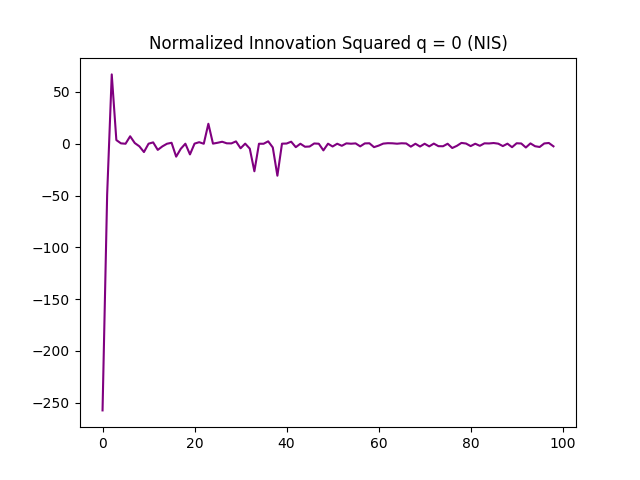
\includegraphics[width=1\linewidth]{./img/nis_0.png}
                    \caption{NIS, q = 0 }
                \end{subfigure}
                \begin{subfigure}{.3\textwidth}  
                    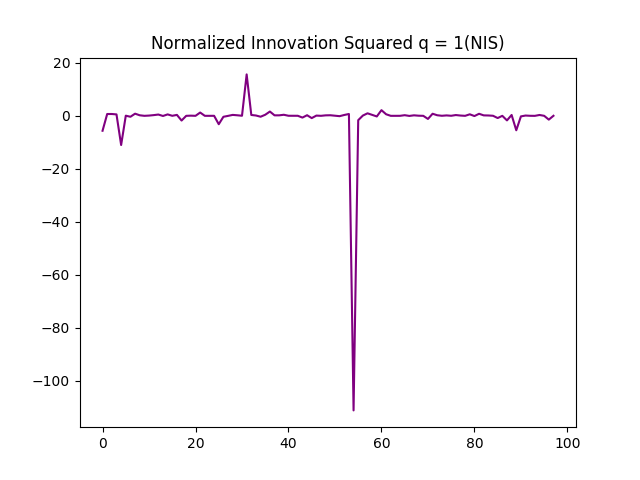
\includegraphics[width=1\linewidth]{./img/nis_1.png}
                    \caption{NIS, q = 1 }
                \end{subfigure}
                \begin{subfigure}{.3\textwidth}
                    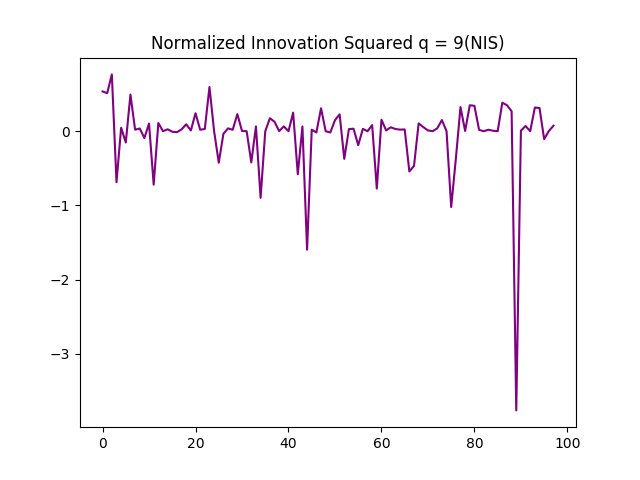
\includegraphics[width=1\linewidth]{./img/nis_9.png}
                    \caption{NIS, q = 9 }
                \end{subfigure}
            \end{subfigure} 
            \caption{NEES \& NIS for different q values [0, 1, 9]}
            \label{fig:error1}
        \end{figure}
        
        Additionally, in the figure \ref{fig:error1} the calculation of the NEES and the NIS is presented for the 3 values of the variance in the process,
        The NEES refers to the precision or difference between the predicted and the real value, based on the covariance of 
        the process. In the sub-figures \textit{(a), (b)} and \textit{(c)} is clear how the NEES increases with more peaks when the variance of
        the process increases. In the other hand the NIS represents the changes in the orientation or more significant changes in the movement of the particle. The NIS 
        drastically changes when there is a significant variation in the acceleration on the motion of the object.
        
        \subsection{Mismatched Model}

        The idea behind of the mismatched model is two different variations both for the filter and for the generation of the data; qf for the filter and qg to
        the generation of the data.

        \begin{figure}[H]
            \begin{subfigure} {.3\textwidth}  
                \centering 
                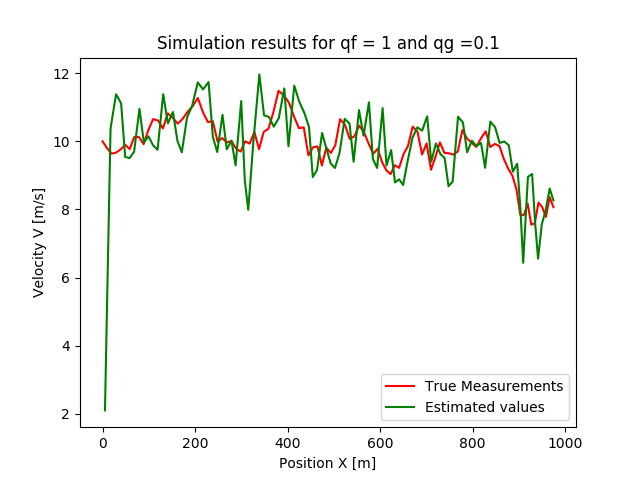
\includegraphics[width=0.9\linewidth]{./img/qf1_qf01.png}
                \caption{qf = 1 \& qg = 0.01 }
            \end{subfigure}
            \begin{subfigure}{.3\textwidth}            
                \centering
                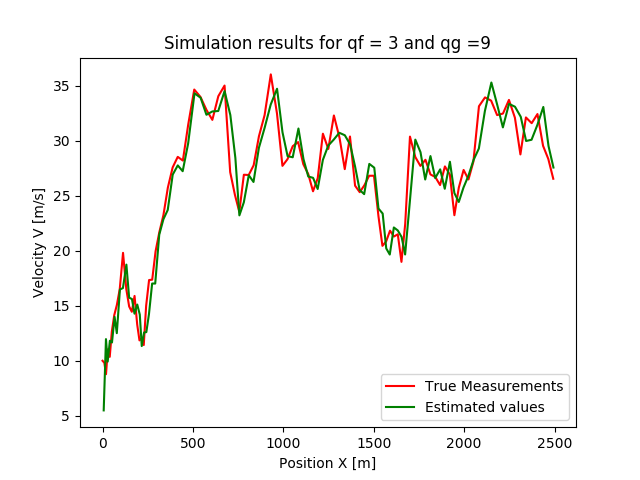
\includegraphics[width=0.9\linewidth]{./img/qf3_qg6.png}
                \caption{qf = 3 \& qg = 9}
            \end{subfigure}    
            \begin{subfigure} {.3\textwidth}         
                \centering
                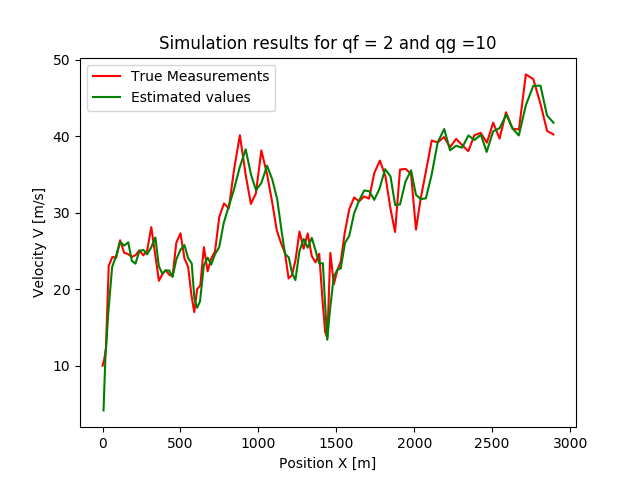
\includegraphics[width=0.9\linewidth]{./img/qf2_qg10.png}
                \caption{qf = 2 \& qg = 10}
            \end{subfigure}
            \caption{Simulation for different for different mismatched q's}
            \label{fig:mismatched}
        \end{figure}

        In the figure \ref{fig:mismatched}, different combinations for the variance in the filter and in 
        the generation of the data were tried. In \textit{(a)} for example the variance for the generation of
        the data is 0.01 which is relatively a small variance in the movement of the particle. On the other hand,
        the variance in the filter is ten times bigger (qf = 1), making harder to predict the movement with a high
        precision. In the graph is clearly notorious that the estimate still try to follows the object trajectory,
        but with a higher error due to the size of the variance in the filter.

        Contrary in \textit{(b)} and \textit{(c)}, the approach was different in the sense that this time the variance
        for the generation of the data would be bigger than the variance of the filter.  The result is a precise prediction 
        with less error compared with the results in \textit{(a)}. The only notable difference is that due to the lower variance 
        in the filter (compared with the variance in the generation of the data) is less sensible to big changes in the 
        movement of the particle. In oder words, the model is filtering "high frequencies" in the measurement of the signal.   

        % p measurement
        \begin{figure}[H]
            \centering 
            \begin{subfigure}{1\textwidth}  
                \begin{subfigure}{.3\textwidth}  
                    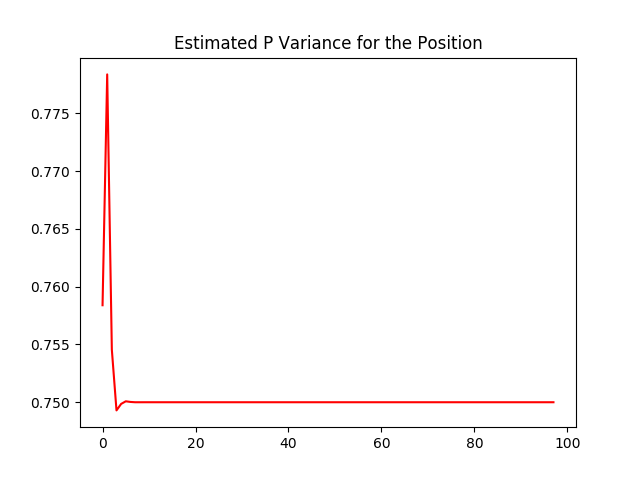
\includegraphics[width=1\linewidth]{./img/p11_qf1.png}
                    \caption{P11 \& q = 0 }
                \end{subfigure}
                \begin{subfigure}{.3\textwidth}  
                    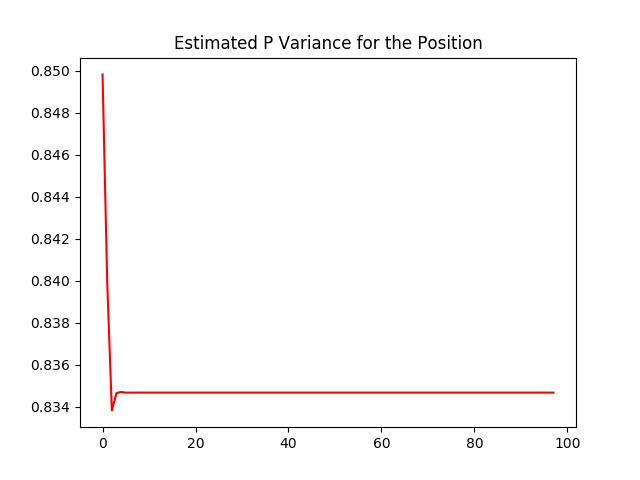
\includegraphics[width=1\linewidth]{./img/p11_qf3.png}
                    \caption{P11 \& q = 1 }
                \end{subfigure}
                \begin{subfigure}{.3\textwidth}  
                    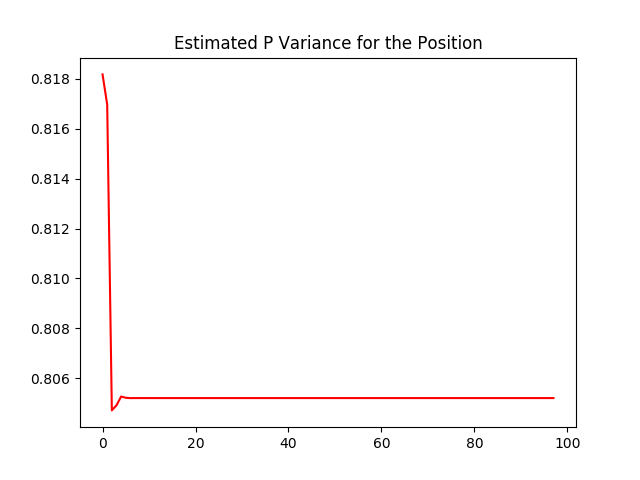
\includegraphics[width=1\linewidth]{./img/p11_qf2.png}
                    \caption[font=0.1mm]{P11 \& q = 9 }
                \end{subfigure}
            \end{subfigure}
            \begin{subfigure} {1\textwidth}    
                \begin{subfigure}{.3\textwidth}  
                    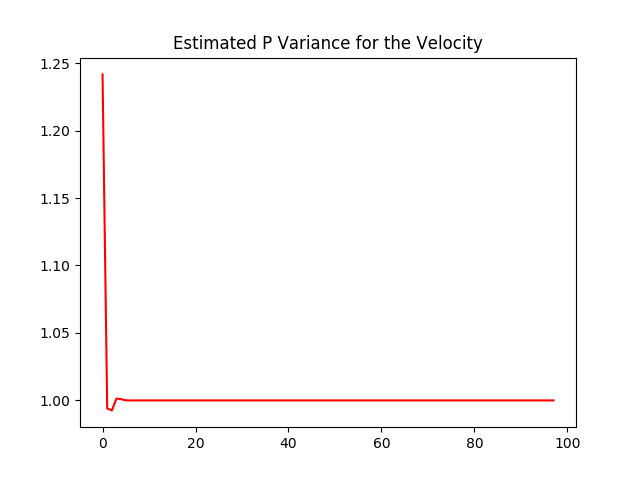
\includegraphics[width=1\linewidth]{./img/p22_qf.png}
                    \caption{P22 \& q = 0 }
                \end{subfigure}
                \begin{subfigure}{.3\textwidth}  
                    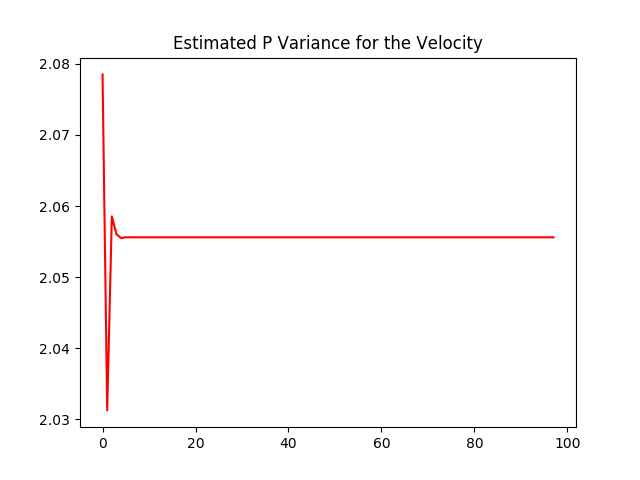
\includegraphics[width=1\linewidth]{./img/p22_q3.png}
                    \caption{P22 \& q = 1 }
                \end{subfigure}
                \begin{subfigure}{.3\textwidth}
                    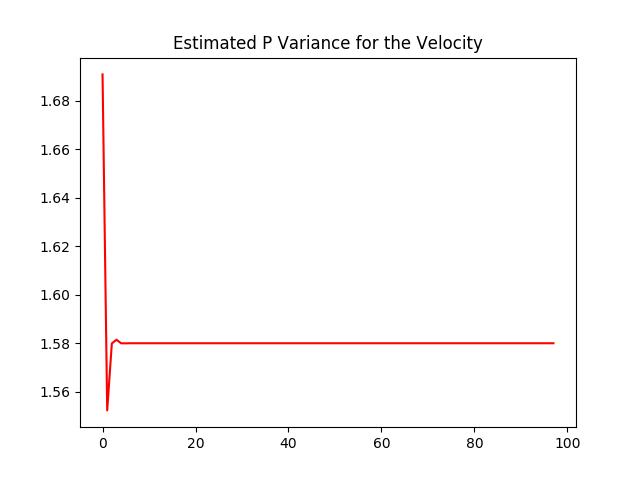
\includegraphics[width=1\linewidth]{./img/p22_qf2.png}
                    \caption{P22 \& q = 9 }
                \end{subfigure}
            \end{subfigure} 
            \caption{State Covariance P for diffetent mismatched q values}
            \label{fig:variancesmis}
        \end{figure}

        % K measurement
        \begin{figure}[H]
            \centering 
            \begin{subfigure}{1\textwidth}  
                \begin{subfigure}{.3\textwidth}  
                    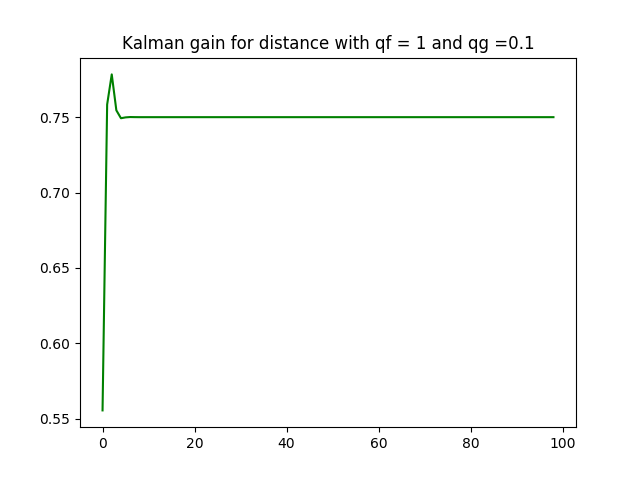
\includegraphics[width=1\linewidth]{./img/k11_qf1.png}
                    \caption{Kp \& q = 0 }
                \end{subfigure}
                \begin{subfigure}{.3\textwidth}  
                    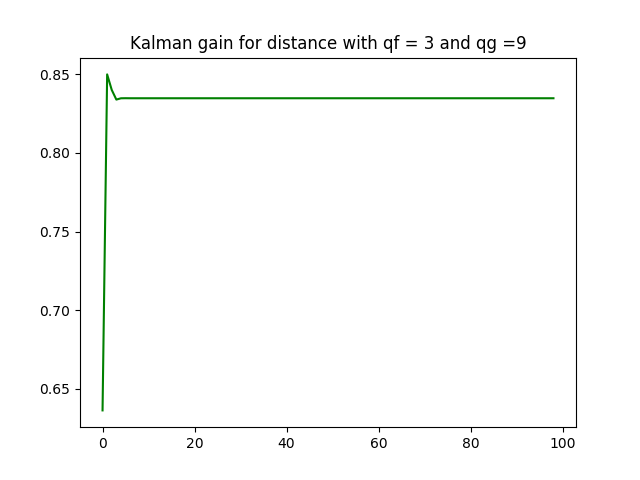
\includegraphics[width=1\linewidth]{./img/k11_q3.png}
                    \caption{Kp \& q = 1 }
                \end{subfigure}
                \begin{subfigure}{.3\textwidth}  
                    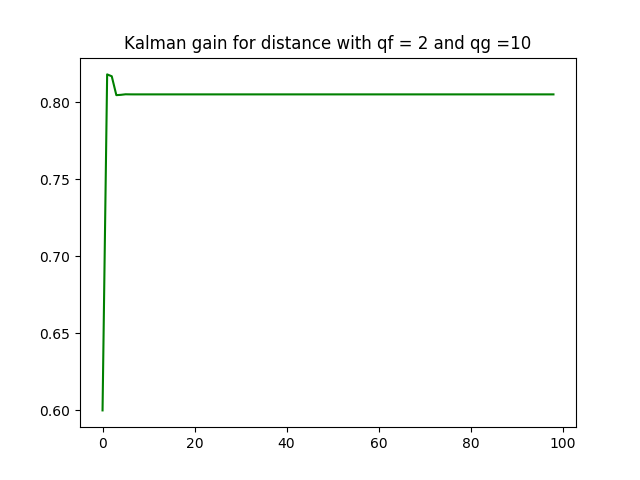
\includegraphics[width=1\linewidth]{./img/k11_qf2.png}
                    \caption[font=0.1mm]{Kp \& q = 9 }
                \end{subfigure}
            \end{subfigure}
            \begin{subfigure} {1\textwidth}    
                \begin{subfigure}{.3\textwidth}  
                    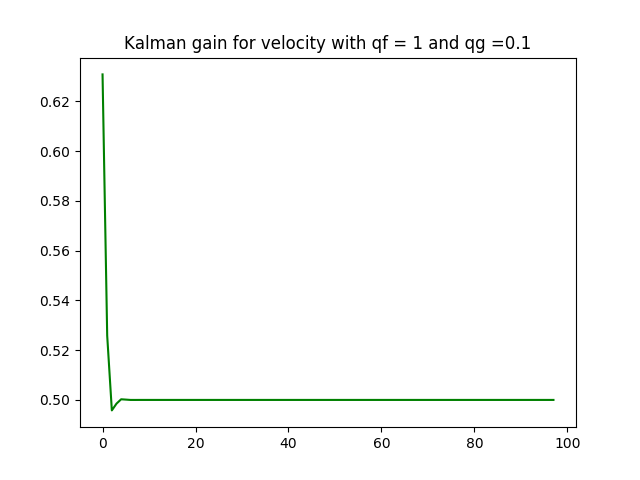
\includegraphics[width=1\linewidth]{./img/k22_qf1.png}
                    \caption{Kv \& q = 0 }
                \end{subfigure}
                \begin{subfigure}{.3\textwidth}  
                    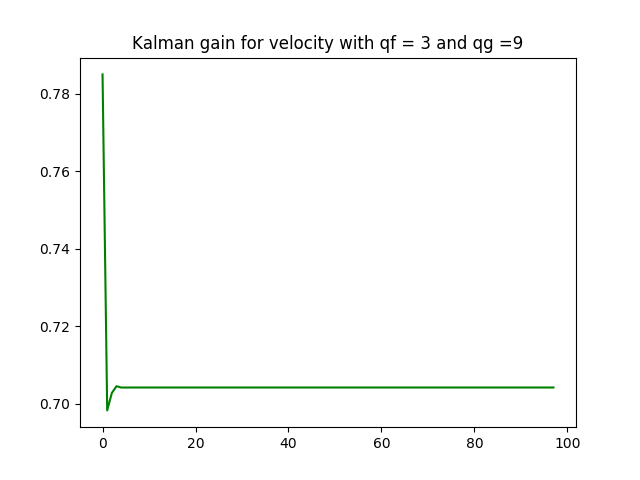
\includegraphics[width=1\linewidth]{./img/k22_q3.png}
                    \caption{Kv \& q = 1 }
                \end{subfigure}
                \begin{subfigure}{.3\textwidth}
                    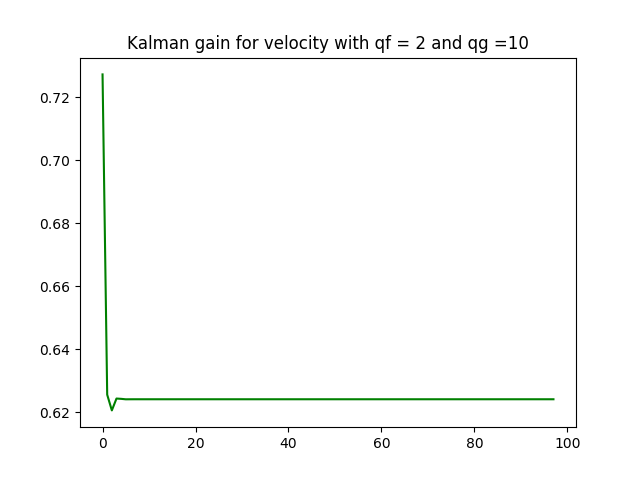
\includegraphics[width=1\linewidth]{./img/k22_qf2.png}
                    \caption{Kv \& q = 9 }
                \end{subfigure}
            \end{subfigure} 
            \caption{Kalman gain for different mismatched q values}
            \label{fig:kalmanmis}
        \end{figure}
        
        The mismatched variances does no affects drastically the state covariance or the Kalman Gain behavior. As is presented
        in the figures \ref{fig:variancesmis} and \ref{fig:kalmanmis}, the shape of the graph is the same as in the matched
        variance scenario (excepting the results with variance equals to zero). The main difference both for the distance and the 
        velocity, is the convergence value for \textit{P} in the model which is usually higher when the variance in the generated data
        is higher than the variance in the filter. 

        \subsection{Monte Carlo Simulation}

        The previous results were done for one run with 100 measurements. Now seeking for a global or mean behavior of the model, the simulation
        is run 50 in a Monte Carlo simulation approach, focusing in the mean error calculation (NEES, NIS and SAC).

        In the figure \ref{fig:mcMatError} the 3 error measurements mentioned before are calculated for different matched q values and
        different \textit{R} values.

        \begin{figure}[H]
            \centering            
            \begin{subfigure} {1\textwidth}    
                \begin{subfigure}{.3\textwidth}  
                    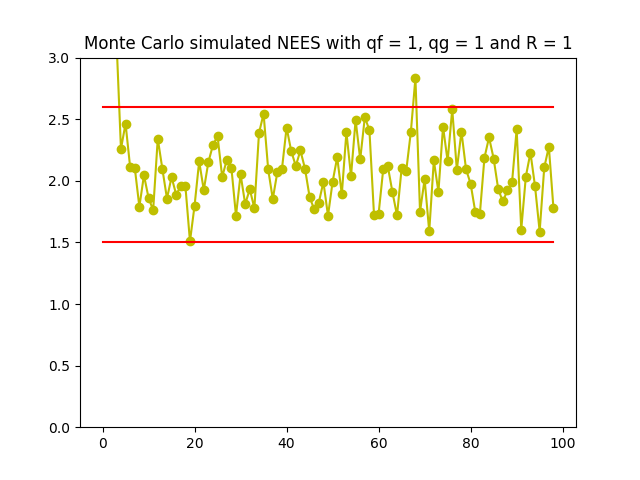
\includegraphics[width=1\linewidth]{./img/mc/nees.png}
                    \caption{NEES qf=1,qg=1, R=1 }
                \end{subfigure}
                \begin{subfigure}{.3\textwidth}  
                    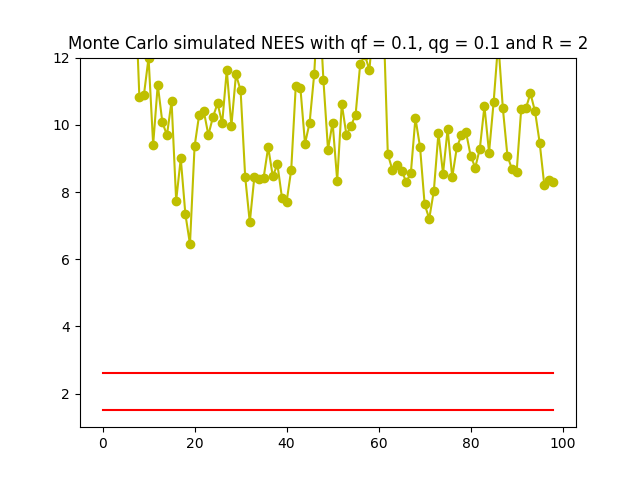
\includegraphics[width=1\linewidth]{./img/mc/nees01r2.png}
                    \caption{NEES qf=0.1,qg=0.1, R=2}
                \end{subfigure}
                \begin{subfigure}{.3\textwidth}
                    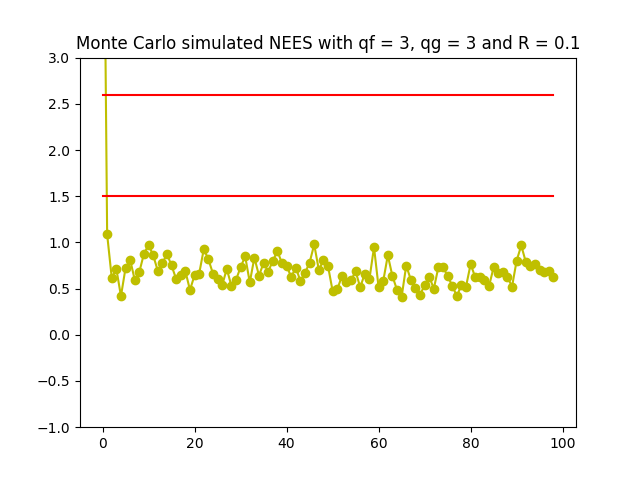
\includegraphics[width=1\linewidth]{./img/mc/nees3r01.png}
                    \caption{NEES qf=3,qg=3, R=0.1 }
                \end{subfigure}
            \end{subfigure} 
            \begin{subfigure} {1\textwidth}    
                \begin{subfigure}{.3\textwidth}  
                    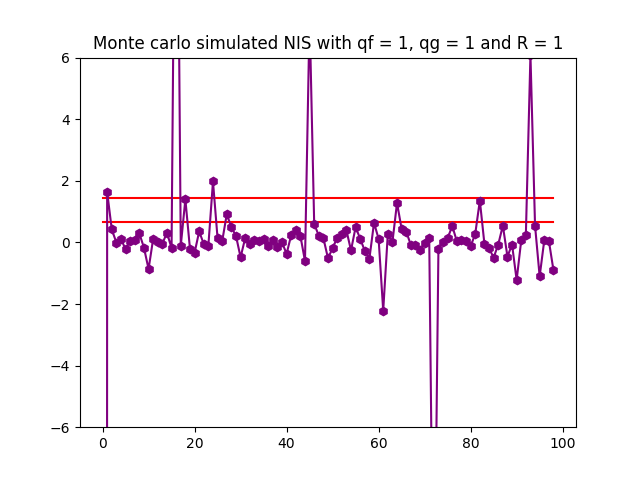
\includegraphics[width=1\linewidth]{./img/mc/nis.png}
                    \caption{NIS qf=1,qg=1, R=1}
                \end{subfigure}
                \begin{subfigure}{.3\textwidth}  
                    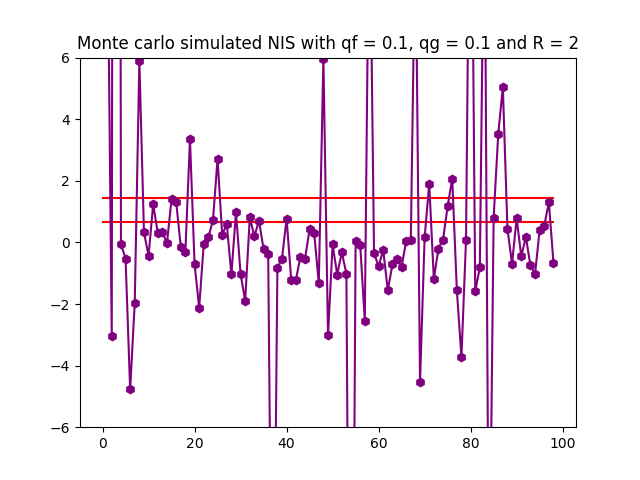
\includegraphics[width=1\linewidth]{./img/mc/nis01r2.png}
                    \caption{NIS qf=0.1,qg=0.1, R=2}
                \end{subfigure}
                \begin{subfigure}{.3\textwidth}
                    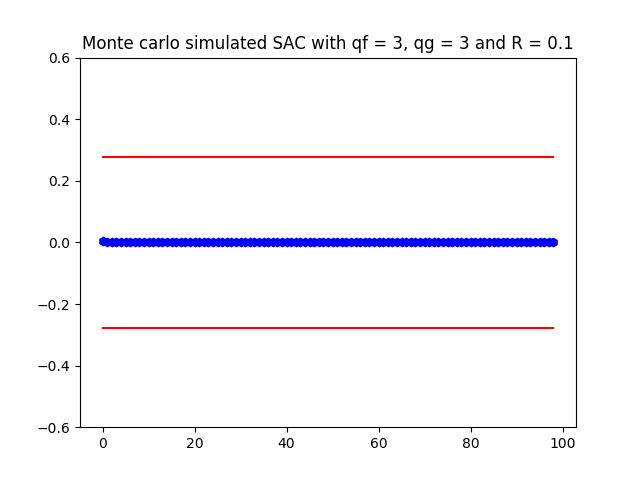
\includegraphics[width=1\linewidth]{./img/mc/nis3r01.png}
                    \caption{NIS qf=3,qg=3, R=0.1}
                \end{subfigure}
            \end{subfigure} 
            \begin{subfigure}{1\textwidth}  
                \begin{subfigure}{.3\textwidth}  
                    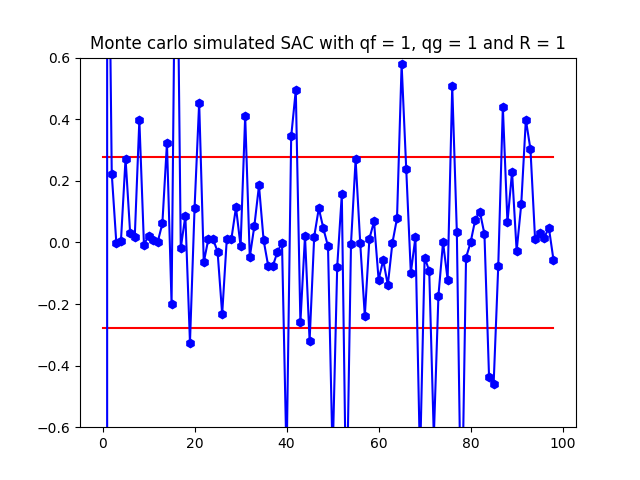
\includegraphics[width=1\linewidth]{./img/mc/sac.png}
                    \caption{SAC qf=1,qg=1, R=1}
                \end{subfigure}
                \begin{subfigure}{.3\textwidth}  
                    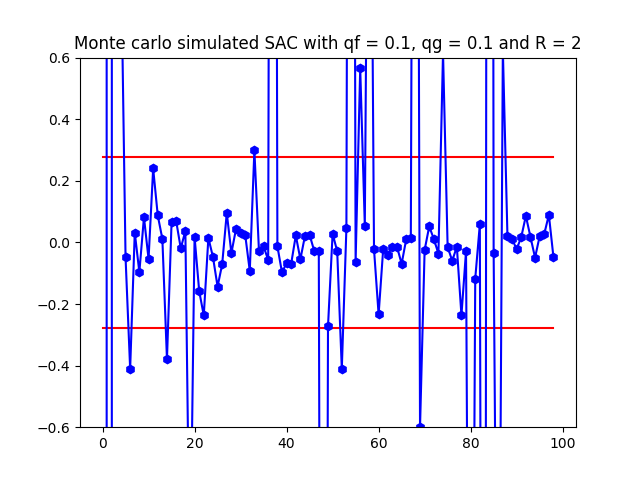
\includegraphics[width=1\linewidth]{./img/mc/sac01r2.png}
                    \caption{SAC qf=0.1,qg=0.1, R=2 }
                \end{subfigure}
                \begin{subfigure}{.3\textwidth}  
                    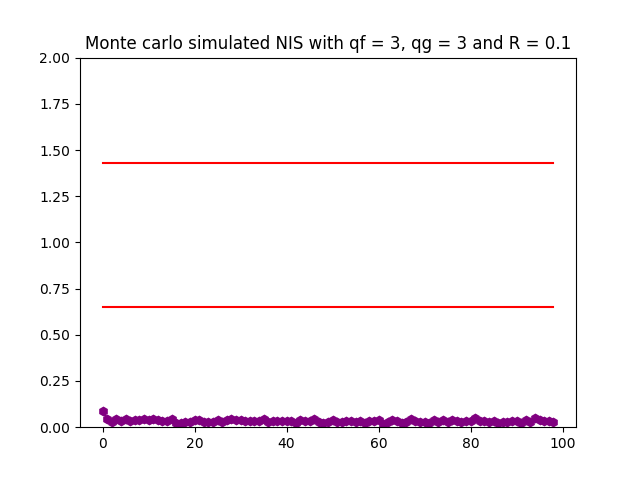
\includegraphics[width=1\linewidth]{./img/mc/sac3r01.png}
                    \caption{ SAC qf=3,qg=3, R=0.1 }
                \end{subfigure}
            \end{subfigure}
            \caption{State Covariance P for diffetent mismatched q values}
            \label{fig:mcMatError}
        \end{figure}
        
        In \textit{(a)} for example, the variance of the process and the sensor is equal to one with error results
        inside of the chi-square distribution boundaries of the problem,excepting for the first values of X while it updates 
        to  the real behavior of the model and one out-lier in the iteration 68.

        Additionally, the NIS and the SAC shows that the innovation error in \textit{(d)} and \textit{(g)} tries to be stable around
        0, but it variates due to the noise in the measurement and the acceleration in the motion of the particle.

        More interesting, it is visible in \textit{(b)} and \textit{(c)} how the noise of the sensor have an important influence in the error (NEES).
        For example, when the noise is "high" in the sensor (R=2), with low variance in the generation of the filer and the data, the error measurement
        is out if the boundaries of the distribution. Differently, when the R is 0.1 with high process variance in the filter and in the generation of the
        data, the prediction does not seems highly affected to reach a considerable level of precision fir the overall model (see \ref{fig:mcMatError} \textit{(c)},\textit{(f)},\textit{(i)}).

        \section{Constant Acceleration Model}

        For the constant acceleration model I decided to play with different values both for q and and for the sensor noise \textit{R}. The 
        approach is also to combine a matched and a mismatched result. 

        \subsection{Matched Model}

        \begin{figure}[H]
            \centering 
            \begin{subfigure}{1\textwidth}  
                \begin{subfigure}{.5\textwidth}  
                    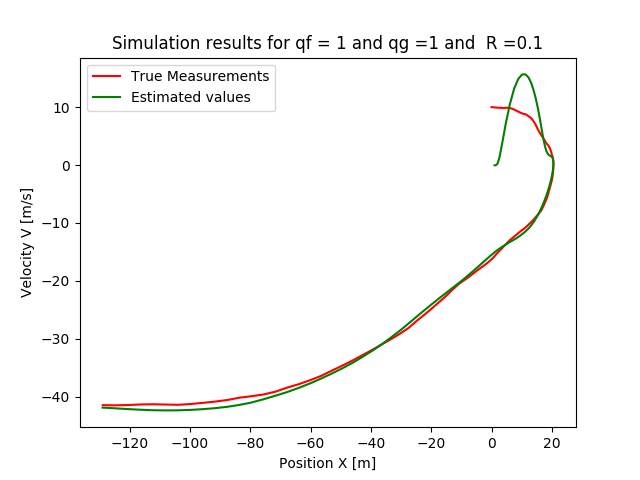
\includegraphics[width=1\linewidth]{./img/acc/qf1_qg1_r01.png}
                    \caption{low q and low R}
                \end{subfigure}
                \begin{subfigure}{.5\textwidth}  
                    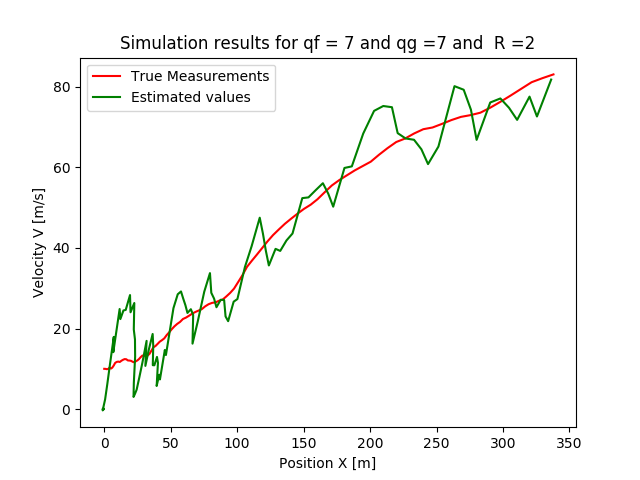
\includegraphics[width=1\linewidth]{./img/acc/qf7_qg7_r2.png}
                    \caption{high q and high R }
                \end{subfigure}                       
            \end{subfigure}
            \caption{Mached variance with constant acceleration}        
            \label{fig:accmat}
        \end{figure}

        In the figure \ref{fig:accmat} is illustrated two different models, \textit{(a)} with a lower error in the 
        sensor for the measurement (\textit{R} = 0.1) and low variance in the filter and in the generation of the data.
        For this case is visible how is harder at the beginning to the model to predict the movement in the negative
        direction, taking more than five iterations to learn the accelerated movement of the object. Additionally, due to
        the small variance in the sensor to measure the position the error in the "steady" state is significantly low as is
        shown in \textit{(a)} and \textit{(b)} in the figure \ref{fig:accmate} both for the NEES and the NIS is high at
        the beginning while the initial position of the particle (position: 0, velocity: 0, acceleration: 0) is updated closely
        to the real state after 17 iterations. From that point on, the error is almost 0.

        Contrary for a value of \textit{qf} and \textit{qg} equals to seven with a higher measurement error, presents a prediction
        which tries to follow the object direction with a low accuracy and a noisy prediction that is visible in the NIS for the figure \ref{fig:accmate}\textit{(d)}
        and in \ref{fig:accmat}\textit{(b)} where the signal variates with a significant error, explained by the higher noise in the
        measurement.

        \begin{figure}[H]
            \centering 
            \begin{subfigure}{1\textwidth}  
                \begin{subfigure}{.5\textwidth} 
                    \centering  
                    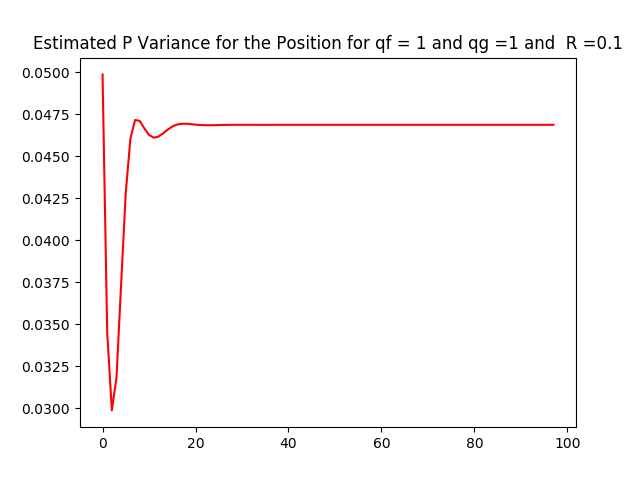
\includegraphics[width=.7\linewidth]{./img/acc/P11_qf1_qg1_r01.png}
                    \caption{ }
                \end{subfigure}
                \begin{subfigure}{.5\textwidth}  
                    \centering 
                    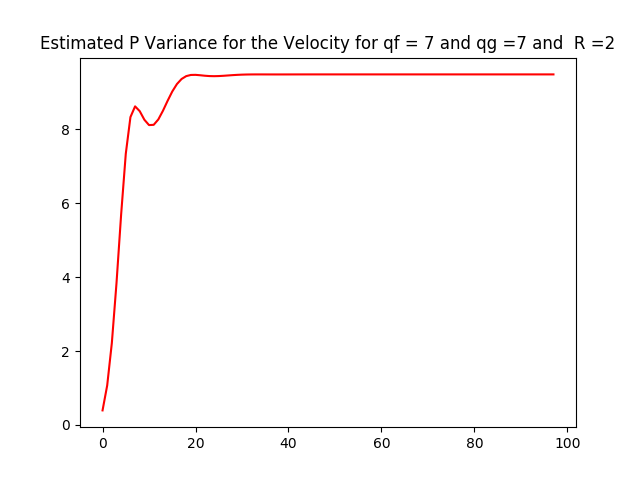
\includegraphics[width=.7\linewidth]{./img/acc/P22_qf7_qg7_r2.png}
                    \caption{}
                \end{subfigure}
            \end{subfigure}
            \caption{P measurements for same qf and qg variance}
            \label{fig:accmatp}
        \end{figure}

        \begin{figure}[H]
            \centering 
            \begin{subfigure}{1\textwidth}  
                \begin{subfigure}{.5\textwidth}  
                    \centering 
                    \includegraphics[width=.7\linewidth]{./img/acc/K11_qf1_qg1_r01.png}
                    \caption{}
                \end{subfigure}
                \begin{subfigure}{.5\textwidth}  
                    \centering 
                    \includegraphics[width=.7\linewidth]{./img/acc/K22_qf7_qg7_r2.png}
                    \caption{ }
                \end{subfigure}                
            \end{subfigure}
            \caption{Kalman gain for different mismatched q values}
            \label{fig:accmatp}
        \end{figure}

        The behavior of the covariance state matrix and the Kalman Gain changes its patter at the start of the predictions
        while it reaches the accelerated movement of the particle. Once this state is predicted, the values converge to one
        value that is mainly affected by the filter variance.

        \begin{figure}[H]
            \centering 
            \begin{subfigure}{1\textwidth}  
                \begin{subfigure}{.5\textwidth}
                    \centering   
                    \includegraphics[width=.6\linewidth]{./img/acc/nees1_qg1_r01.png}
                    \caption{ }
                \end{subfigure}
                \begin{subfigure}{.5\textwidth}  
                    \centering 
                    \includegraphics[width=.6\linewidth]{./img/acc/nis1_qg1_r01.png}
                    \caption{}
                \end{subfigure}
                \begin{subfigure}{.5\textwidth} 
                    \centering  
                    \includegraphics[width=.6\linewidth]{./img/acc/nees7_qg7_r2.png}
                    \caption{}
                \end{subfigure}
                \begin{subfigure}{.5\textwidth} 
                    \centering  
                    \includegraphics[width=.6\linewidth]{./img/acc/nis7_qg7_r2.png}
                    \caption{}
                \end{subfigure}                
            \end{subfigure}
            \caption{Error measurements for same qf and qg variance}
            \label{fig:accmate}
        \end{figure}

        \subsection{Mismatched Model}

        For the mismatched model on the other hand, it is more complex to decided which values to try to have interesting
        prediction model to study. At the end as is presented in the figure \ref{fig:accmis} I decided two use two scenarios,
        one with a "higher" filter variance and "high" measurement variance, and  a second one with "low" process variance in the
        filter and still a "high" \textit{R}.

        In the first simulated case, is visible in \textit{(a)} how the noise in the measurement of the position and the filter process
        variance does not allow the model to produce a accurate prediction. The error and the noise influence is also notable in the NIS
        results in the figure \ref{fig:accmise} \textit{(b)}.

        \begin{figure}[H]
            \centering 
            \begin{subfigure}{1\textwidth}  
                \begin{subfigure}{.5\textwidth}  
                    \centering 
                    \includegraphics[width=1\linewidth]{./img/acc/qf3_qg1_r2.png}
                    \caption{}
                \end{subfigure}
                \begin{subfigure}{.5\textwidth}
                    \centering   
                    \includegraphics[width=1\linewidth]{./img/acc/qf01_qg4_r2.png}
                    \caption{}
                \end{subfigure}
            \end{subfigure}
            \caption{low qf and high R}
            \label{fig:accmis}
        \end{figure}

        More interesting in the figure \ref{fig:accmis}\textit{(b)}  even when the noise measurement stays "high" and the variance in the generation
        of the data (acceleration) for the movement is also "high", but the variance of the process in the filter (qf) remains "low", the process is 
        able to filter the "high frequencies" of noise in the process, providing an accurate and precise prediction when it is compared with \textit{(a)}.

        In terms of error, is also distinguishable \ref{fig:accmise}\textit{(d)} how the noise is significantly reduce.
        \begin{figure}[H]
            \centering 
            \begin{subfigure}{1\textwidth}  
                \begin{subfigure}{.5\textwidth}
                    \centering   
                    \includegraphics[width=.6\linewidth]{./img/acc/P11_qf3_qg1_r2.png}
                    \caption{}
                \end{subfigure}
                \begin{subfigure}{.5\textwidth}  
                    \centering 
                    \includegraphics[width=.6\linewidth]{./img/acc/P22_qf01_qg4_r2.png}
                    \caption{}
                \end{subfigure}
            \end{subfigure}
            \caption{P measurements for different mismatched q values}
            \label{fig:accmisp}
        \end{figure}

        \begin{figure}[H]
            \centering 
            \begin{subfigure}{1\textwidth}  
                \begin{subfigure}{.5\textwidth}  
                    \centering 
                    \includegraphics[width=.7\linewidth]{./img/acc/K11_qf3_qg1_r2.png}
                    \caption{}
                \end{subfigure}
                \begin{subfigure}{.5\textwidth}  
                    \centering 
                    \includegraphics[width=.7\linewidth]{./img/acc/K22_qf01_qg4_r2.png}
                    \caption{}
                \end{subfigure}
            \end{subfigure}
            \caption{Kalman gain for different mismatched q values}
            \label{fig:accmisk}
        \end{figure}

        P and consequently K presents a small variation at the beginning while the convergence state is reached, staying similarly to the previous
        studied results.

        \begin{figure}[H]
            \centering 
            \begin{subfigure}{1\textwidth}  
                \begin{subfigure}{.5\textwidth}  
                    \centering 
                    \includegraphics[width=.5\linewidth]{./img/acc/nees3_qg1_r2.png}
                    \caption{}
                \end{subfigure}
                \begin{subfigure}{.5\textwidth}  
                    \centering                     
                    \includegraphics[width=.5\linewidth]{./img/acc/nis3_qg1_r2.png}
                    \caption{}
                \end{subfigure}
                \begin{subfigure}{.5\textwidth}  
                    \centering 
                    \includegraphics[width=.5\linewidth]{./img/acc/nees01_qg4_r2.png}
                    \caption{}
                \end{subfigure}
                \begin{subfigure}{.5\textwidth} 
                    \centering  
                    \includegraphics[width=.5\linewidth]{./img/acc/nis01_qg4_r2.png}
                    \caption{}
                \end{subfigure}
            \end{subfigure}               
            \caption{Error for different mismatched q values}
            \label{fig:accmise}
        \end{figure}

        \subsection{Monte Carlo Simulation}

        For the mismatched model, is a smoother movement where witha good variance in the filterm the process is able to predic the position
        close to the real behavior of thr particle.

        \begin{figure}[H]
            \centering 
            \begin{subfigure}{1\textwidth}  
                \begin{subfigure}{.3\textwidth}  
                    \includegraphics[width=1\linewidth]{./img/mc/acc/nees1_qg5_r1.png}
                    \caption{qf=1, qg=5 \& R=1}
                \end{subfigure}
                \begin{subfigure}{.3\textwidth}  
                    \includegraphics[width=1\linewidth]{./img/mc/acc/nees1_qg5_r01.png}
                    \caption{qf=1, qg=5 \& R=0.1}
                \end{subfigure}
                \begin{subfigure}{.3\textwidth}  
                    \includegraphics[width=1\linewidth]{./img/mc/acc/nees1_qg01_r01.png}
                    \caption{qf=1, qg=0.1 \& R=1 }
                \end{subfigure}
            \end{subfigure}
            \begin{subfigure} {1\textwidth}    
                \begin{subfigure}{.3\textwidth}  
                    \includegraphics[width=1\linewidth]{./img/mc/acc/nis1_qg5_r1.png}
                    \caption{qf=1, qg=5 \& R=1}
                \end{subfigure}
                \begin{subfigure}{.3\textwidth}  
                    \includegraphics[width=1\linewidth]{./img/mc/acc/nis1_qg5_r01.png}
                    \caption{qf=1, qg=5 \& R=0.1 }
                \end{subfigure}
                \begin{subfigure}{.3\textwidth}
                    \includegraphics[width=1\linewidth]{./img/mc/acc/nis1_qg01_r01.png}
                    \caption{qf=1, qg=0.1 \& R=0.1}
                \end{subfigure}
            \end{subfigure} 
            \begin{subfigure} {1\textwidth}    
                \begin{subfigure}{.3\textwidth}  
                    \includegraphics[width=1\linewidth]{./img/mc/acc/sac1_qg5_r1.png}
                    \caption{qf=1, qg=0.1 \& R=1}
                \end{subfigure}
                \begin{subfigure}{.3\textwidth}  
                    \includegraphics[width=1\linewidth]{./img/mc/acc/sac1_qg5_r01.png}
                    \caption{qf=1, qg=5\& R=0.1}
                \end{subfigure}
                \begin{subfigure}{.3\textwidth}
                    \includegraphics[width=1\linewidth]{./img/mc/acc/sac1_qg01_r01.png}
                    \caption{qf=1, qg=0.1 \& R=0.1}
                \end{subfigure}
            \end{subfigure} 
            \caption{State Covariance P for diffetent mismatched q values}
            \label{fig:mcMisError}
        \end{figure}

        In the figure \ref{fig:mcMisError} the NEES do not stays inside the boundaries when the variance is mismatched for the
        generation of the data and for the filter. furthermore, the model is sensitive to the changes in the filter; for example,
        when the variance in the sensor (R) goes from 1 to 0.1, the NIS and the SAC dramatically changes because the model is perceptible
        of changes in the acceleration or movement of the particle. 
        
        In other words, The NEES responds faster to the changes in the process and the NIS and SAC variates with small changes in the noise of
        the sensor measuring the position of the particle.

        \bibliography{report}
        \bibliographystyle{ieeetr}
        \nocite{*}


    \end{document}